\chapter{Navegación autónoma en seguimiento de rutas 3D}\label{cap.desarrollo}
\hspace{1cm} En este capítulo se describ el sistema diseñado y desarrollado para conseguir los objetivos planteados, utilizando la infraestructura mencionada anteriormente y como se ha implementado.

\hspace{1cm} La solución ha sido un algoritmo de navegación autónoma sobre el cual se dará una visión global. A continuación, se explicará en detalle su diseño y el funcionamiento de cada uno de los componentes que lo integran. Por la complejidad inherente del problema, en este sistema ha sido necesario adaptar e integrar partes de software ya existentes previamente así como desarrollar otros bloques nuevos.

%\hspace{1cm} Para explicar todos los pasos primero se dara un vistazo al diseño globalmente para posteriormente explicar cada uno de los modulos individualmente y así poder conocer todos ellos en detalle.

\section{Diseño}
\hspace{1cm} El objetivo de este algoritmo es que un drone realice un comportamiento completamente autónomo desde el despegue, hasta el aterrizaje, pasando por recorrer de una ruta tridimensional previamente definida. Todo esto basándose únicamente en balizas de apoyo visual y en los motores de sus hélices. Es decir, el vuelo completamente autónomo de un drone mediante visión artificial y control de posición.

\hspace{1cm} En la aplicación final se diferencian dos partes principales: por un lado, tenemos el componente encargado de estimar la posición mediante algoritmos de visión por computador y por otro lado, tenemos el componente que se encarga del control del drone tomando las decisiones del movimiento según la etapa en la que se encuentre.

\hspace{1cm} En la Figura \ref{fig:Esquema representativo.} se puede ver una explicación de las entradas y salidas de flujos de información. También se pueden observar los ficheros que son imprescindibles en cada módulo para su correcto funcionamiento. Esta imagen nos da una idea del funcionamiento global de la aplicación, cada módulo es un proceso independiente que funciona iterativamente y como toda la comunicación entre procesos se lleva a cabo mediante la biblioteca ICE. A continuación vamos a explicar el comportamiento de cada módulo de una forma breve para tener una visión panorámica de la aplicación completa.

\begin{figure}[H]
	\begin{center}
		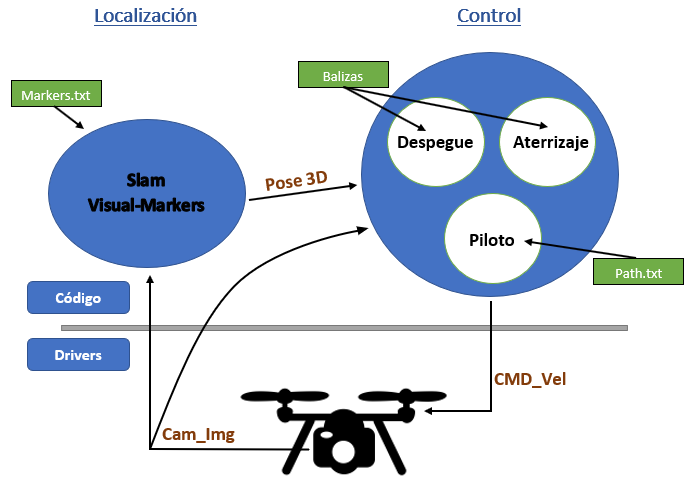
\includegraphics[width=1\textwidth]{imag/IMG80.PNG}
				\caption{Diseño del sistema de navegación autónoma en 3D.}
		\label{fig:Esquema representativo.}	
	\end{center}
\end{figure}

\hspace{1cm} El nodo de localización \texttt{Slam VisualMarkers} recibe las imágenes que le proporciona el drone y envía los datos en forma de Pose3D(x,y,z,q0,q1,q2,q3) al componente de control. Este componente comienza analizando la imagen recibida en busca de la presencia de marcadores AprilTags. Si no los encuentra devuelve el número 0 como indicador de ello, en cambio si encuentra alguna envía por el interfaz ICE cuántas ha encontrado y aplica cálculos de geometría proyectiva para estimar la posición tridimensional de la cámara con respecto a cada una de las balizas. A continuación realiza una fusión espacial, aplicando un filtro basado en pesos y una fusión temporal, mediante un filtro de Kalman para elaborar su estimación de posición 3D. Finalmente, la estimación calculada se envía al componente de navegación o control mediante una interfaz ICE.

\hspace{1cm} El nodo de control recibe la imagen de la cámara del drone y las posiciones estimadas, envía estos datos a las etapas internas que lo necesiten y según en la etapa en la que se encuentre genera una serie de órdenes de velocidades para los motores que envía al drone vía interfaz ICE para conseguir el objetivo. Según la etapa ese objetivo puede ser despegar, aterrizar o seguir una ruta.

\hspace{1cm} A continuación vamos a explicar cada módulo con mayor profundidad, nuestro mayor desarrollo en este TFG fue la creación de un algoritmo de pilotaje que mejorase los anteriores tanto en precisión de seguimiento de rutas como en tiempo de realización de estas rutas, por lo que será el aparado en el que más nos centraremos. Sin embargo, al ser un TFG de integración también explicaremos los módulos en los que nos hemos basado y hemos ajustado para su correcto funcionamiento en el algoritmo final. 

\section{Componente de Autolocazalización} 
%\hspace{1cm} Este nodo lo desarrollo originalmente Alberto López, luego fue refactorizado por Samuel Martín para integrar una capa de comunicaciones mediante interfaces ICE, también añadió métodos para la conversión entre cuaterniones y ángulos de Euler, debido a que la aplicación original utilizaba los ángulos de Euler y la interfaz Pose3D, cuaterniones, posteriormente Manuel Zafra la actualizo para jderobot e hizo los primeros pasos de navegación de drones utilizando esta autolocalización. Por último Felipe Pérez ha cambiado los ficheros de configuración para que sea una herramienta que funcione utilizando únicamente librerías que vienen en JdeRobot por si sola, sin depender de QtCreator y su compilador \textit{qmake}, también está creando la nueva infraestructura en ROS para que se pueda utilizar tanto en ICE como en esta, con la ventaja de que en ROS tendrá nuevos marcadores como el número de balizas detectadas para poder hacer estudios de precisión y marcas temporales para saber cuándo entran las balizas en la aplicación y así caracterizar mejor el error de posición. 

\hspace{1cm} En cuanto al componente \texttt{Slam-VisualMarkers} está formado por el módulo principal \textit{Main-Window} que interconecta el resto de módulos e implementa una interfaz gráfica de usuario. El método \textit{ProcessImage} contenido en \textit{CameraManager} se ocupa de procesar la imagen en 2D capturada por la cámara y buscar en ésta la presencia de marcadores además de estimar la posición 3D con respecto a éstos. Es imprescindible el fichero \texttt{Markers.txt} que contiene toda la información necesaria de cada marcador: id, tamaño y posición absoluta 3D.

\hspace{1cm} Para localizar los marcadores en la imagen se hace uso del método de detección ofrecido por la biblioteca AprilTags. Este método se aplica a una versión en escala de grises de la imagen obtenida y tiene como salida un array en el que figuran todos los marcadores encontrados en la imagen. Una vez el array de marcadores detectados es generado, se aplican una serie de operaciones geométricas. Estas operaciones devuelven la posición relativa de una cámara calculada estableciendo la correspondencia entre los puntos 2D de la imagen y los correspondientes puntos 3D de la baliza. De esta forma se obtienen los vectores de translación y rotación del marcador con respecto a la cámara.

\hspace{1cm} Finalmente, la matriz que contiene la posición de la cámara con respecto al mundo se obtiene multiplicando la matriz calculada, posición relativa del marcador con respecto a la cámara, y la matriz de posición del mundo con respecto al marcador. 

\begin{figure}[H]
	\begin{center}
		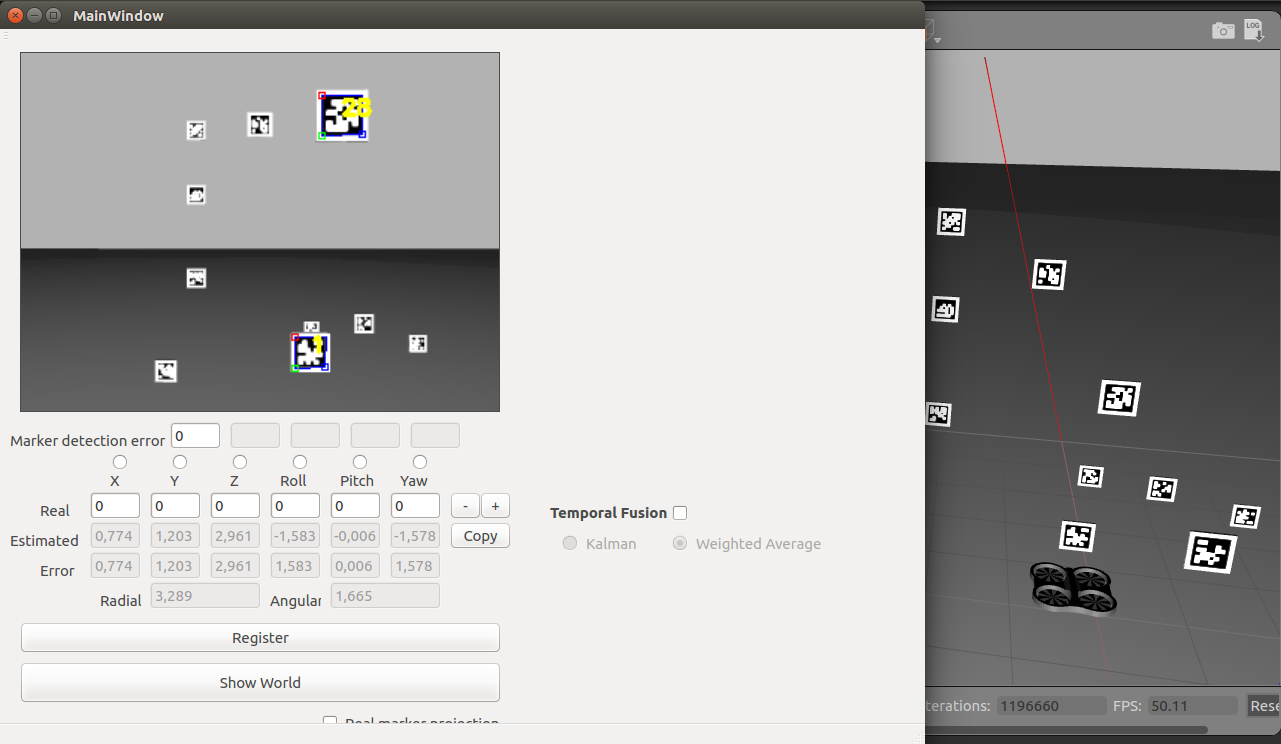
\includegraphics[width=0.85\textwidth]{imag/IMG35.png}
				\caption{Entorno del componente \texttt{Slam VisualMarkers}}
		\label{fig:Ejemplo Slam VisualMarkers.}	
	\end{center}
\end{figure}

\hspace{1cm} Las posiciones 3D estimadas para cada marcador observado en la imagen son almacenadas en un array y se fusionan mediante un filtro por pesos (fusión espacial). Este filtro asigna diferentes pesos a cada estimación basándose en la distancia a la cámara, de forma que a los marcadores más cercanos se les asigna un peso mayor. En esta combinación ponderada, para los ángulos de rotación hay una operación especial, ya que no pueden ser sumados de la misma forma que las coordenadas lineales. 

\hspace{1cm} Por último, después de aplicar la fusión espacial, la aplicación original daba opción a aplicar una fusión temporal. Esta fusión puede llevarse a cabo de dos maneras, que se elige por configuración: mediante un nuevvo filtro por pesos, o mediante la aplicación de un Filtro de Kalman \cite{FiltroKalman}.

\hspace{1cm} Con la nueva herramienta, además de calcular la posición tridimensional, también se incorpora el número de balizas detectadas en la imagen en las que se basa esa estimación y una marca temporal. Esto proporciona una indicación de la fiabilidad de la
estimación y en que momento se produce tal estimación.

\section{Componente de Control basado en estados}
\hspace{1cm} Todo el algoritmo de navegación autónoma se ha basado en un componente de control basado en estados, este componente se ha realizado con la herramienta de \texttt{Visual States}, la cual nos ha servido tanto para la creación del código, como para la integración de las diferentes partes del sistema en un solo programa. 

\hspace{1cm} \texttt{Visual States} tiene la capacidad de crear estados, donde dentro se escribe el código que se ejecuta cuando está activo, los cuales recorre mediante transiciones que pueden ser temporales o condicionales. Esto permite al programador centrarse en la escritura del algoritmo porque de la conexión entre estados se encarga la herramienta. Además, tiene otras secciones donde se especifican las constantes y las funciones que una vez creadas se pueden utilizar en todos los estados y transiciones, pudiendo así conectar y llevar un seguimiento de lo que ocurre en cada estado. Por último, \texttt{Visual States} ofrece la sección de las librerías, en la cual se introducen aquellas de las que depende tu programa, y el apartado de configuración, donde irán los diferentes enlaces a los interfaces de comunicación que hayamos utilizado. 

%\hspace{1cm} Es la parte en la que más nos hemos centrado y que más hemos conseguido desarrollar dentro del algoritmo, ya que para nosotros es la parte más importante. Se podría decir que se trata de un piloto el cual realiza las tareas de pilotaje del drone. Hemos dividido el pilo según los datos que recibe de la interface de VisualStates.

\begin{figure}[H]
	\begin{center}
		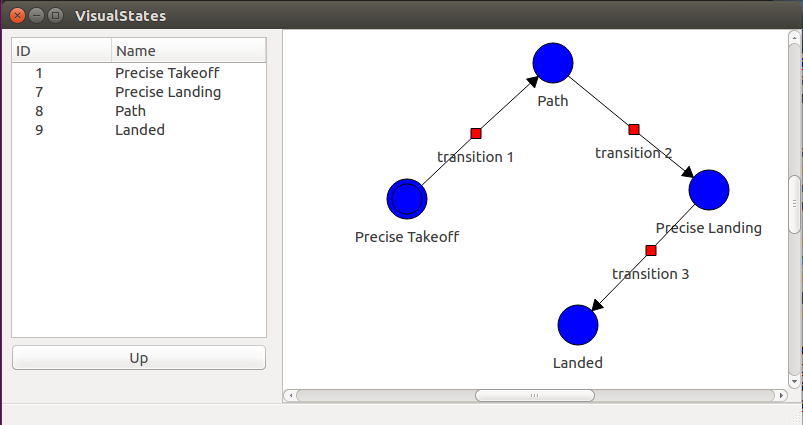
\includegraphics[width=0.8\textwidth]{imag/IMG60.png}
				\caption{Diseño en cuatro estados de la navegación visual autónoma para seguimiento de rutas en 3D, usando la herramienta VisualStates.}
		\label{fig:Esquema VisualStates.}	
	\end{center}
\end{figure}

\hspace{1cm} En la Figura \ref{fig:Esquema VisualStates.} se observan los diferentes estados y transiciones en los que se ha dividido la aplicación. El primer estado es el de \textit{Precise Takeoff} en el cual el drone despega y se posiciona sobre la baliza arlequinada de despegue, a continuación pasa por la primera transción en la cual se dejan de enviar ordenes de control para que el dron se estabilice y se cambia de la cámara inferior a la frontal. El siguiente estado es el de \textit{Path} donde entra la herramienta de autolocalización para seguir la ruta establecida. Una vez concluida la ruta entra la transición dos en la cual se decide si el dron debe seguir ralizando la ruta desde el inicio o pasar al modulo de aterrizaje. Éste seria el siguiente módulo \textit{Precise Landing} en el cual se vuelve a cambiar la cámara a la inferior para buscar la baliza arlequinada de aterrizaje, una vez encontrada se procede al centrado y al descenso, hasta un punto en el cual la baliza ocupa la totalizad del objetivo de la cámara, que es cuando se para a la transición tres, donde se ponen todas las velocidades a cero menos la de descenso. Por último de llega al estado de \textit{Landed} que significa que el drone desciende verticalmente hasta que al cámara esta sobre la baliza y se paran todos los motores. 

\begin{figure}[H]
	\begin{center}
		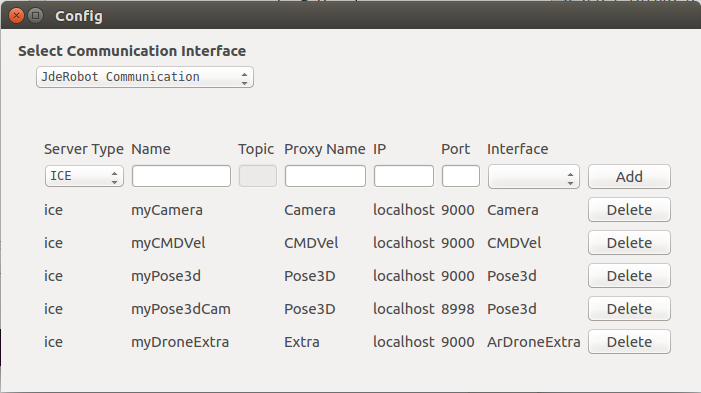
\includegraphics[width=0.8\textwidth]{imag/IMG70.png}
				\caption{Interfaces de comunicación de Visual States.}
		\label{fig:Esquema interfaces VisualStates.}	
	\end{center}
\end{figure}

La Figura \ref{fig:Esquema interfaces VisualStates.} nos muestra los diferentes interfaces sobre los que se basa la aplicación, que cuadran con los explicados en la figura \ref{fig:Esquema representativo.}, estos son integrados por la herramienta para crear una correcta comunicación con el drone y así conseguir el correcto comportamiento de navegación desarrollado. 

\subsection{Estado de despegue}
\hspace{1cm} Para este componente se ha utilizado el trabajo que realizó Jorge Vela en su TFG \cite{JorgeVela} refactorizándolo y acoplándolo dentro de nuestro módulo de pilotaje en \texttt{Visual States}. Es el estado activo nada más arrancar la aplicación, el diseño de este algoritmo es un proceso basado en adquisición-procesado-envío de órdenes a los motores. La adquisición de los datos se realiza mediante los sensores de imágenes del drone. Estos datos sensoriales serán recogidos para su procesamiento y tras esto se enviarán las instrucciones al drone para que las ejecute. El sensor utilizado en este estado ha sido la cámara.

\hspace{1cm} El lugar de despegue del drone es una baliza arlequinada previamente definida \ref{fig:Baliza.}. Esta baliza es un cuadrado que en su interior tiene cuatro cuadrantes, dos verdes, y dos azules. Esta baliza se diseñó así para que sea difícil confundirla con otro objeto, pues de ser una baliza simple se podrían confundir los colores, además lo que busca el software será la cruceta que forman estos cuatro cuadrados y el punto central de ésta.

\begin{figure}[H]
	\begin{center}
		
\includegraphics[width=0.4\textwidth]{imag/IMG33.png}
				\caption{Baliza utilizada en Gazebo.}
		\label{fig:Baliza.}	
	\end{center}
\end{figure}

\hspace{1cm} En el \textbf{despegue} se sitúa el drone sobre una baliza sobre la cual tiene que estabilizarse. De esta forma, al despegar detecta ésta y trata de centrarse, evitando así que se desvíe por factores externos como una ligera brisa o derivas en el propio movimiento, quedándose en la situación correcta. Para realizar el movimiento de centrarse en la baliza se ha utilizado un control PD (proporcional y derivativo) en el cual centra la cruceta de la baliza arlequinada con el punto central de la cámara, cuando esto se consigue y la baliza es una proporción de la imagen total se pasa al siguiente módulo que sería el del piloto.

\subsection{Estado de seguimiento de ruta por puntos de paso}
\hspace{1cm} Como se puede observar en la imagen \ref{fig:Esquema VisualStates.} el algoritmo de este componente se activa en el estado de Path y se encarga de que el drone siga una ruta. Hemos desarrollado dos algoritmos diferentes según el tipo de trayectoria que se le introduzca, si es una trayectoria de subobjetivos como puntos relativamente separados es el \textbf{Piloto por puntos de paso}. Si en cambio la trayectoria es una ruta de puntos prácticamente continuos entonces se trataría del \textbf{Piloto por trayectoria}. Ambos algoritmos se basan en la posición tridimensional del drone. Para el control hemos utilizado los tipos de datos de JdeRobot \textit{Pose3D} los cuales nos devuelven tanto la posición del drone como su orientación en el espacio, mediante los cuaterniones o los Ángulos de Euler según lo que necesitemos. Estos datos son proporcionados por la estimación del componente de posición de \texttt{Slam VisualMarkers}. Y nuestro algoritmo de navegación devuelve una serie de velocidades que va enviando al cuadricóptero mediante la función \textit{CMDVel()}.

\hspace{1cm} Por su sencillez de pilotaje vamos a explicar primero el \textbf{Piloto por puntos de paso}. Este control de pilotaje se centra en el movimiento direccional únicamente, es decir, para que el drone alcance el punto de paso al que debe llegar no variará prácticamente ninguno de sus ángulos de Euler, tan solo se moverá sobre los ejes x,y,z.

\hspace{1cm} Como el movimiento será únicamente direccional en coordenadas cartesianas tan solo hay que calcular el vector que apunta desde la posición del cuadricóptero hasta el siguiente punto de ruta que se desea alcanzar: 

\[Pose3D = (P_{x}, P_{y}, P_{z})\hspace{1cm};\hspace{1cm}Beacon = (B_{x}, B_{y}, B_{z})\]
\[\overrightarrow{V}_{x} = P_{x} - B_{x}\hspace{0.5cm};\hspace{0.5cm}\overrightarrow{V}_{y} = P_{y} - B_{y}\hspace{0.5cm};\hspace{0.5cm}\overrightarrow{V}_{z} = P_{z} - B_{z}\]

\hspace{1cm} Una vez calculado este vector entre las posiciones, lo multiplicamos por un coeficiente regulador que reduce los valores hasta que éstos se encuentren dentro del rango de velocidades del drone y una vez alcanzado este rango se pasan los valores por una función que compruebe que las velocidades máximas no exceden las permisibles por \texttt{Slam VisuaMarkers} para la detección y análisis de balizas: 

\begin{lstlisting}[backgroundcolor=\color{gray!15}]
    if math.fabs(Vx) > MaxVx :
        Vx = MaxVx * np.sign(Vx)
    if math.fabs(Vy) > MaxVy :
        Vy = MaxVx * np.sign(Vy)
    if math.fabs(Vz) > MaxVz :
        Vz = MaxVx * np.sign(Vz)        
\end{lstlisting}

\hspace{1cm} Con este método de control de navegación por posición nos aseguramos de que el drone alcanza el punto que queremos adecuadamente y a medida que se va acercando a él, para que la aproximación sea exacta, al reducirse el vector se reducirá la velocidad alcanzando la baliza con total exactitud. Una vez se alcanza la baliza se busca cual es la siguiente en la lista y se vuelve a realizar el proceso, así hasta alcanzar todas ellas.

\subsection{Estado de seguimiento de ruta por trayectoria continua}
\hspace{1cm} En cuanto al \textbf{Piloto por trayectoria continua} se creó para permitir un control mucho más fino del movimiento del drone y así seguir
trayectorias más angulosas y con variaciones más fuertes. Lo primero fue crear las rutas que posteriormente seguiría el drone, como éstas debían ser largas con giros y con puntos muy consecutivos se creó en Python la función que nos permitiese crear éstas según la separación entre puntos de ruta que considerásemos necesaria, la ruta va en un fichero como secuencia de puntos muy próximos entre sí: 
\begin{lstlisting}[backgroundcolor=\color{gray!15}]
i=0
a=0
if i == 0:
    archivo = open('pos.txt','w')
    archivo.write('  x     y     z    roll   pitch   yaw \n')
    i = i+1
b = time.clock()
pos_sim = self.pose.getPose3d()
    if ((b - a) > time_write):
        archivo.write(str(pos_sim.x)+' ')
        archivo.write(str(pos_sim.y)+' ')
        archivo.write(str(pos_sim.z)+' ')
        archivo.write(str(pos_sim.roll)+' ')
        archivo.write(str(pos_sim.pitch)+' ')
        archivo.write(str(pos_sim.yaw)+' ')
        archivo.write(str(b)+'\n')
        a = b 
\end{lstlisting}

\hspace{1cm} A diferencia del \textit{Piloto por puntos de paso} éste seguirá los puntos orientándose siempre en la dirección entre la posición y el siguiente punto, para ello tendremos que variar la velocidad angular en torno al eje Z, modificando por tanto el ángulo de yaw del drone y de esta forma conseguir orientarlo de la forma más rápida hasta el siguiente punto de la ruta. Conforme se fue investigando se descubrió que permitir al drone realizar pequeñas variaciones en la velocidad lineal del eje Y permitía un aproximación a los puntos efectiva y precisa, por lo que se optó por incluir también la variación de la velocidad en el eje Y.

\hspace{1cm} Para el cálculo de las velocidades lineales Vx, Vy y Vz se seguirán los mismos pasos que en el \textbf{Piloto por puntos de paso} pero variaremos los coeficientes de corrección para que las velocidades lineales sean parejas a la nueva velocidad angular Wz. Esta velocidad angular se calculará mediante las funciones de predicción de posición. 

\hspace{1cm} El primer paso de esa predicción es calcular la distancia horizontal que recorrerá el drone hasta la siguiente iteración del algoritmo. La distancia se obtiene multiplicando la velocidad horizontal obtenida anteriormente por el tiempo que transcurre entre dos iteraciones: \(d_{\psi} = v_{x} * \Delta_{t}\).

\hspace{1cm} Para predecir la posición del cuadricóptero debemos tener en cuenta el ángulo de giro con respecto al eje Z del drone en ese instante. Ya que en el estándar de Pose3D la orientación se indica en cuaterniones, haremos una conversión para conocer el ángulo de Euler mediante la siguiente ecuación:

\[ \Psi_{z} = arctan^{2}\left( \frac{2*q_{0}*q_{3}+q_{1}*q_{2}}{1-2*(q_{2}^{2}+q_{3}^{2})}\right) \]
 
\hspace{1cm} Una vez obtenido el ángulo $\Psi_{z}$ sacamos la posición que predecimos sólo en X e Y ya que la variación en Z no influye en cálculo del ángulo de giro de yaw.

\[ X_{f} = d_{\psi} * cos \Psi_{z} + x_{pose} \] 
\[ Y_{f} = d_{\psi} * sin \Psi_{z} + y_{pose} \]

\hspace{1cm} Ahora calculamos el error de ángulo, que es la diferencia entre el ángulo actual y el ángulo sobre el eje Z existente entre el drone y el punto de ruta, $\Psi_{e}$ Teniendo el ángulo se calcula una velocidad angular a partir de la distancia horizontal al punto, $d_{H}$, y la velocidad lineal actual, $v_{x}$.
 
\[\Psi_{path} = arctan \left(\frac{V_{y}}{V_{x}}\right)  \hspace{0.5cm};\hspace{0.5cm}\Psi_{e} = \Psi_{path} - \Psi_{z} \]

\[d_{H} = \sqrt{V_{x}^{2} + V_{y}^{2}} \hspace{0.5cm};\hspace{0.5cm} \omega_{e} =  \dfrac{\Psi_{e}}{d_{H}/v_{x}}\]

\hspace{1cm} La velocidad angular dependerá entonces de la velocidad angular calculada y de un factor de corrección que viene dado por la relación entre el error lateral predicho $L_{fe}$ y la velocidad horizontal. Este factor está multiplicado por una constante $K_{g}$, que es la ganancia de corrección del giro.

\[ L_{fe} = cos\Psi_{z}*(Y_{path}-Y_{f}) - sin\Psi_{z}*(X_{path}-X_{f}) \]
\[ \omega_{z} = \omega_{e} + K_{g} * (L_{fe}/v_{x})\]

\hspace{1cm} Por último, una vez obtenida la velocidad angular $\omega_{z}$ ajustamos la velocidad en el eje Y, $v_{y}$, a partir de ésta.

\hspace{1cm} Una vez obtenidas las tres velocidades que se van a enviar al drone, las velocidades horizontales $v_{x}$ $v_{y}$, la velocidad vertical $v_{z}$ y velocidad angular $\omega_{z}$ se envían al drone mediante una llamada al método \textit{SendCMDVel(vx,vy,vz,wz)} de Interfaces, que se ocupa de mandar las órdenes decididas al cuadricóptero.

\subsection{Estado de aterrizaje}
\hspace{1cm} Una vez el cuadricóptero termina la ruta establecida, éste procede a la siguiente etapa que es el \textbf{aterrizaje}, el cual se divide en dos partes, primero la búsqueda de la baliza de aterrizaje y luego el centrado de la misma y el descenso sobre ésta. 

\hspace{1cm} En cuanto a la búsqueda, sigue una navegación en espiral creciente de forma que irá rastreando la zona ampliando su giro de forma continua, hasta que detecte una baliza arlequinada. Si no se detecta una baliza, continuará el algoritmo de búsqueda, aumentando la amplitud de las espirales. Cuando se detecte, dejará el movimiento en espiral y buscará que coincida el centro de la baliza con el centro de la imagen de la cámara.  Para realizar el movimiento de centrarse en la baliza se ha utilizado un control PD, ya que la percepción visual de la baliza es la misma que en el estado de despegue.  

\hspace{1cm} Por último, una vez coincide la cruceta de la baliza con el centro de la imagen, comienza a descender de forma constante a la vez que va centrando imagen por si el drone se desvía por algún factor externo. Cuando el área que detecta la baliza es mayor al área de la cámara, en ese momento el drone desciende hasta  posarse en el suelo, entonces para los motores y el estado cambia a al estado final de \textit{"Landed"}.

\begin{figure}[H]
	\begin{center}
		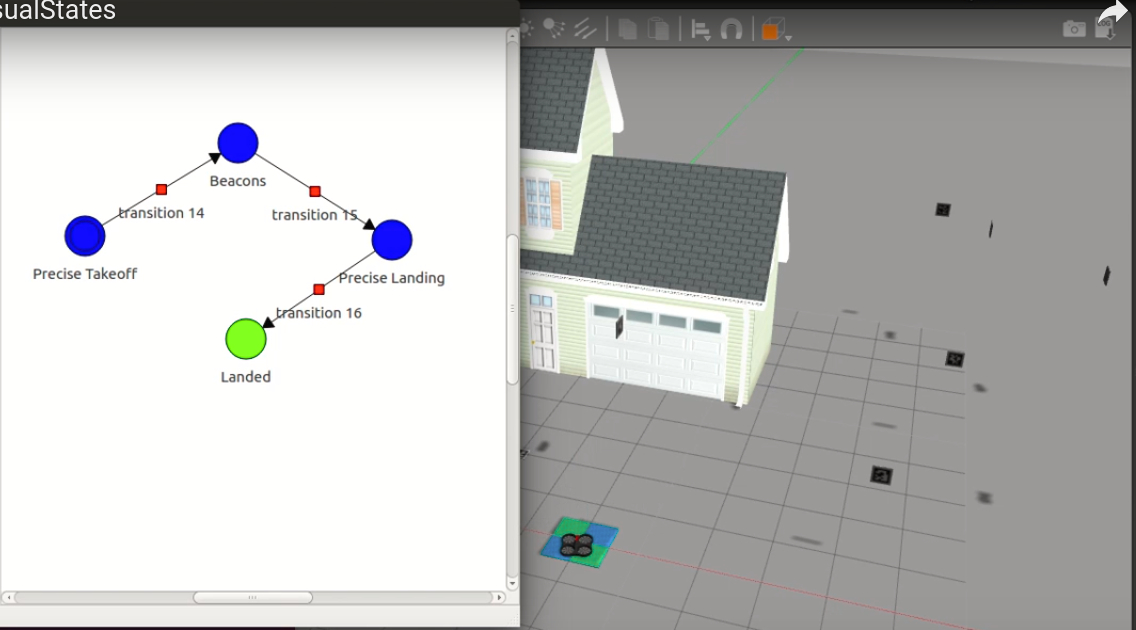
\includegraphics[width=0.9\textwidth]{imag/IMG34.png}
				\caption{Ejemplo de los estados en Visual States}
		\label{fig:Ejemplo Visual States.}	
	\end{center}
\end{figure}